\subsection{Clustering}
\label{Res_Clu}

Using the simpleKMeans clustering algorithm in Weka results in the graph in figure \ref{fig:clusters} (a larger version can be seen in figure \ref{fig:largeClusters} in the appendix on page \pageref{fig:largeClusters}, and the clusters and their centroids in section \ref{A_kmr_clusters} on page \pageref{A_kmr_clusters} in the appendix). The x-axis is the name of the country, the y-axis is the year and the color of the cross is the cluster the country belongs to at that time.

\begin{figure}[h!]
  \centering
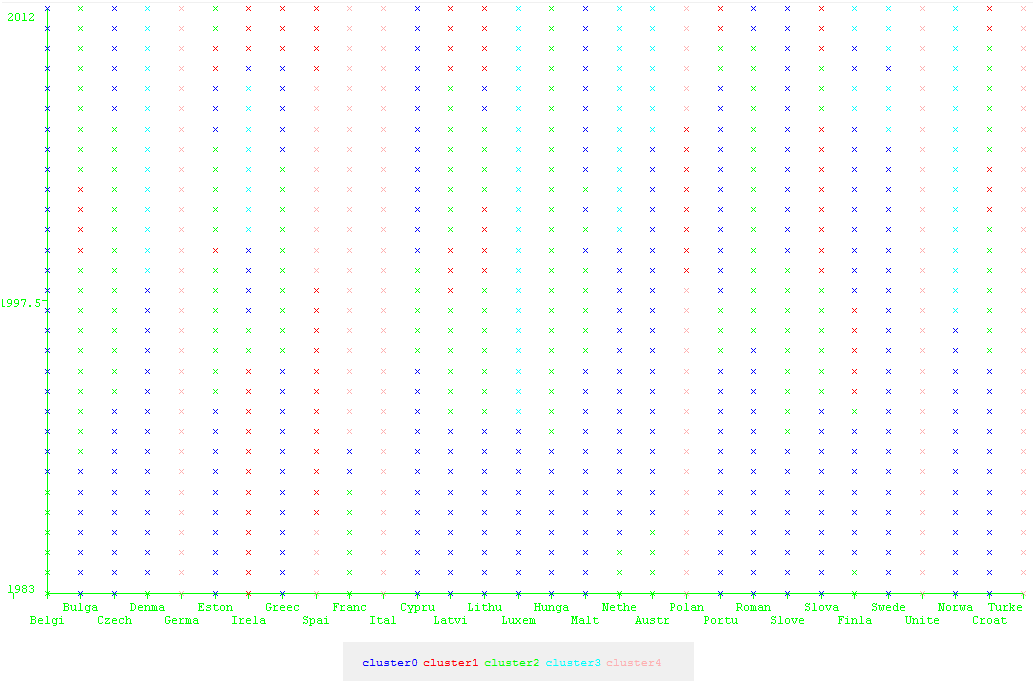
\includegraphics[width=\textwidth]{Appendix/Images/kMeans}
\caption{Graphical representation of what clusters the countries belong to at what year}
\label{fig:clusters}
\end{figure}

From the graph, we can observe that there are three countries that - assuming "often" means seven or more times - change cluster often. They are Estonia, Malta and Finland. Their behaviour is somewhat eratic, however:
\begin{itemize}
	\item Estonia starts in cluster \#0, then changes to cluster \#2 for a long while with one year in cluster \#1. Lastly it moves from cluster \#0 to cluster \#1 to cluster \#2 over the span of a few years.

	\item Malta has a period where it switches between cluster \#0 and \#2 each year over a period of five years, indicating that it is right on the border of the cluster during that period.

	\item Finland moves through all clusters but cluster \#4, though it stays in cluster \#0 for a bit more than half the years.
\end{itemize}

There are also four countries that are the complete opposite, as they never change what cluster they are in. They are Germany, Italy, United Kingdom and Turkey and never leave cluster \#4. Furthermore, they are in the same cluster, which indicates that it is a very stable cluster and they are very stable countries.

Inserting USA into the cluster data (with data from 2011) puts USA in cluster \#4\footnote{See appendix \ref{A_kmr_usa} on \pageref{A_kmr_usa} for the output}. This means that USA is in the same cluster as Germany, France, Italy, United Kingdom and Turkey, which means that USA is more similar to them than any other European country at that time.